%! Author = Nhan Huynh
%! Date = 03/11/2021

% Preamble
\documentclass{../tuda-beamer}

% Title information
\authors{Simon Hock}
\authors{Nhan Huynh}
\date{03. November 2021}

% Document
\begin{document}

    \maketitle

    \begin{frame}{Überblick}
        \tableofcontents
    \end{frame}


    \section{Organisatorisches}
    \begin{frame}{Organisatorisches}
        \begin{itemize}
            \item Themensprechstunde und Präsenzsprechstunden: Plätze verfügbar!
            \item Offene Fragen zu Korrekturen? Siehe Ankündigung!
            \begin{itemize}
                \item Ansprechpartner kontaktieren
                \item Bitte zuerst die Musterlösung ansehen und ggf. Tutorentests ausführen und
                erst dann nachfragen!
            \end{itemize}
            \item Forum - Themenwünsche
            \begin{itemize}
                \item Einzelne Themen werden dann zu Beginn in der Präsenzsprechstunde besprochen
            \end{itemize}
        \end{itemize}
    \end{frame}

    \begin{frame}[c]
        \begin{figure}[h]
            \centering
            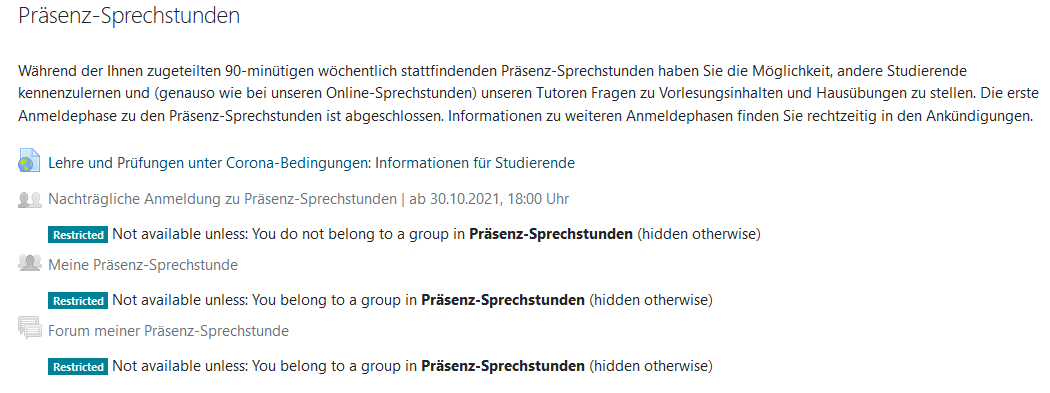
\includegraphics[width=\linewidth]{graphics/pss_forum.png}
            \caption{Abschnitt Sprechstunden, Betreuung und Zusammenarbeit}
        \end{figure}
    \end{frame}

    \begin{frame}[c]
        \begin{figure}[h]
            \centering
            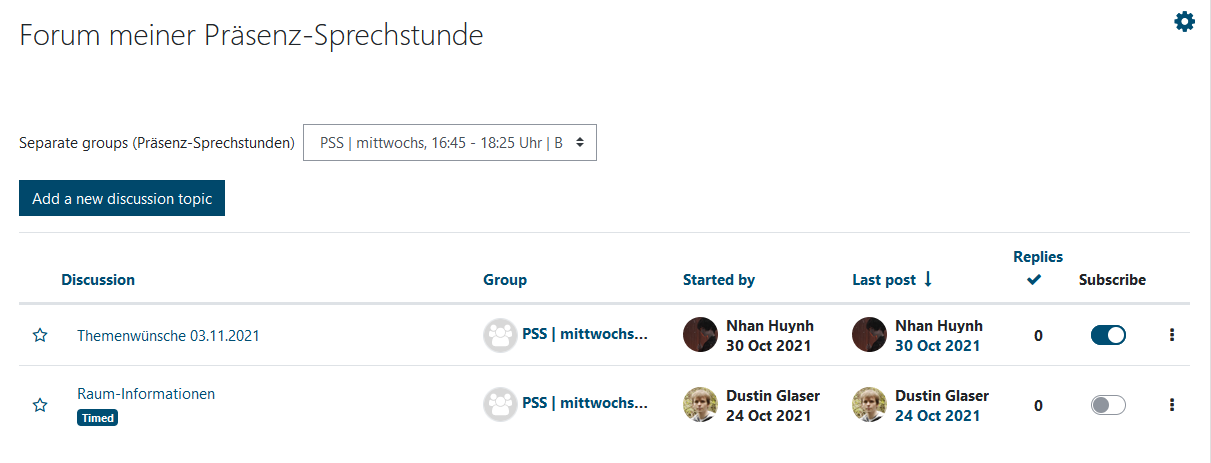
\includegraphics[width=\linewidth]{graphics/pss_themenwuensche.png}
            \caption{Präsenzsprechstunden - Forum}
        \end{figure}
    \end{frame}


    \section{Methoden}
    \begin{frame}{Methoden}
        \begin{itemize}
            \item (Objekt-)Methoden definieren das Verhalten eines Objektes
            \item Formaler Aufbau:

            \begin{center}
                Zugriffsmodifikator\(^*\)  \inlinejava{static}\(^*\)  Rückgabetyp
                Bezeichner(Parameter\(^*\));
            \end{center}

            \begin{itemize}
                \item \(^*\) (Asterisk): Optional
                \item Parametern werden ebenfalls auch als Argumente bezeichnet
            \end{itemize}
            \item Mehr Informationen findet ihr im Check + Prepare Kurs!
            \begin{itemize}
                \item Thematische Zusammenfassung -  Java Fortgeschritten
            \end{itemize}
        \end{itemize}
    \end{frame}

    \begin{frame}
        \lstinputlisting[style=Java, title=Bauplan eines Autos in Java - Klasse Car]{codes/Car.java}
    \end{frame}

    \begin{frame}{Mathematische Analogie: Funktionen}
        \begin{itemize}
            \item \enquote{Funktionen sind eine Beziehung zwischen zwei Mengen, die jedem Element
            der einen Menge genau ein Element der anderen Menge zuordnet.}
            \item Beispiel: \(f(x) = x^2, x \in \mathbb{N}\)

            \lstinputlisting[style=Java, title=Funktion \(f\) in Java]{codes/function_square.java}
        \end{itemize}
    \end{frame}


    \section{Random Number Generator}
    \begin{frame}{Random Number Generator}
        \begin{itemize}
            \item Generiert pseudozufällige Zahlen
            \item Basisklasse: \inlinejava{Random}
            \item Subklassen: \inlinejava{SecureRandom}, \inlinejava{ThreadLocalRandom}
            \item Hausübung: Verwendung von \inlinejava{ThreadLocalRandom}
        \end{itemize}
    \end{frame}

    \begin{frame}{Die Würfel sind gefallen!}
        \begin{itemize}
            \item Simulieren Sie einen Würfelwurf, wobei die Augenzahlen zwischen 1 und 6 (beides
            inklusiv) sind. Dabei soll der Würfel fair sein, das heißt alle Augenzahlen sollen mit
            identischer Wahrscheinlichkeit auftreten.
        \end{itemize}

        \lstinputlisting[style=Java, title=Würfelwurf-Simulation in Java]{codes/diceRoll.java}
    \end{frame}


    \section{Arbeitsphase}
    \begin{frame}[c]{Arbeitsphase}
        \begin{center}
            \textbf{\LARGE Selbstständiges Arbeiten}
        \end{center}
    \end{frame}
\end{document}
